\documentclass[twoside]{book}

% Packages required by doxygen
\usepackage{fixltx2e}
\usepackage{calc}
\usepackage{doxygen}
\usepackage[export]{adjustbox} % also loads graphicx
\usepackage{graphicx}
\usepackage[utf8]{inputenc}
\usepackage{makeidx}
\usepackage{multicol}
\usepackage{multirow}
\PassOptionsToPackage{warn}{textcomp}
\usepackage{textcomp}
\usepackage[nointegrals]{wasysym}
\usepackage[table]{xcolor}

% Font selection
\usepackage[T1]{fontenc}
\usepackage[scaled=.90]{helvet}
\usepackage{courier}
\usepackage{amssymb}
\usepackage{sectsty}
\renewcommand{\familydefault}{\sfdefault}
\allsectionsfont{%
  \fontseries{bc}\selectfont%
  \color{darkgray}%
}
\renewcommand{\DoxyLabelFont}{%
  \fontseries{bc}\selectfont%
  \color{darkgray}%
}
\newcommand{\+}{\discretionary{\mbox{\scriptsize$\hookleftarrow$}}{}{}}

% Page & text layout
\usepackage{geometry}
\geometry{%
  a4paper,%
  top=2.5cm,%
  bottom=2.5cm,%
  left=2.5cm,%
  right=2.5cm%
}
\tolerance=750
\hfuzz=15pt
\hbadness=750
\setlength{\emergencystretch}{15pt}
\setlength{\parindent}{0cm}
\setlength{\parskip}{0.2cm}
\makeatletter
\renewcommand{\paragraph}{%
  \@startsection{paragraph}{4}{0ex}{-1.0ex}{1.0ex}{%
    \normalfont\normalsize\bfseries\SS@parafont%
  }%
}
\renewcommand{\subparagraph}{%
  \@startsection{subparagraph}{5}{0ex}{-1.0ex}{1.0ex}{%
    \normalfont\normalsize\bfseries\SS@subparafont%
  }%
}
\makeatother

% Headers & footers
\usepackage{fancyhdr}
\pagestyle{fancyplain}
\fancyhead[LE]{\fancyplain{}{\bfseries\thepage}}
\fancyhead[CE]{\fancyplain{}{}}
\fancyhead[RE]{\fancyplain{}{\bfseries\leftmark}}
\fancyhead[LO]{\fancyplain{}{\bfseries\rightmark}}
\fancyhead[CO]{\fancyplain{}{}}
\fancyhead[RO]{\fancyplain{}{\bfseries\thepage}}
\fancyfoot[LE]{\fancyplain{}{}}
\fancyfoot[CE]{\fancyplain{}{}}
\fancyfoot[RE]{\fancyplain{}{\bfseries\scriptsize Generated on Tue Jan 10 2017 14\+:07\+:37 for My Project by Doxygen }}
\fancyfoot[LO]{\fancyplain{}{\bfseries\scriptsize Generated on Tue Jan 10 2017 14\+:07\+:37 for My Project by Doxygen }}
\fancyfoot[CO]{\fancyplain{}{}}
\fancyfoot[RO]{\fancyplain{}{}}
\renewcommand{\footrulewidth}{0.4pt}
\renewcommand{\chaptermark}[1]{%
  \markboth{#1}{}%
}
\renewcommand{\sectionmark}[1]{%
  \markright{\thesection\ #1}%
}

% Indices & bibliography
\usepackage{natbib}
\usepackage[titles]{tocloft}
\setcounter{tocdepth}{3}
\setcounter{secnumdepth}{5}
\makeindex

% Hyperlinks (required, but should be loaded last)
\usepackage{ifpdf}
\ifpdf
  \usepackage[pdftex,pagebackref=true]{hyperref}
\else
  \usepackage[ps2pdf,pagebackref=true]{hyperref}
\fi
\hypersetup{%
  colorlinks=true,%
  linkcolor=blue,%
  citecolor=blue,%
  unicode%
}

% Custom commands
\newcommand{\clearemptydoublepage}{%
  \newpage{\pagestyle{empty}\cleardoublepage}%
}


%===== C O N T E N T S =====

\begin{document}

% Titlepage & ToC
\hypersetup{pageanchor=false,
             bookmarks=true,
             bookmarksnumbered=true,
             pdfencoding=unicode
            }
\pagenumbering{roman}
\begin{titlepage}
\vspace*{7cm}
\begin{center}%
{\Large My Project }\\
\vspace*{1cm}
{\large Generated by Doxygen 1.8.9.1}\\
\vspace*{0.5cm}
{\small Tue Jan 10 2017 14:07:37}\\
\end{center}
\end{titlepage}
\clearemptydoublepage
\tableofcontents
\clearemptydoublepage
\pagenumbering{arabic}
\hypersetup{pageanchor=true}

%--- Begin generated contents ---
\chapter{R\+E\+A\+D\+M\+E}
\label{md_README}
\hypertarget{md_README}{}
\#\+Humrarnas projektarbete -\/ Garbage Collector

\subsubsection*{Medlemmar\+:}


\begin{DoxyItemize}
\item Adam Inersjö -\/ Teamansvarig
\item Daniel Ågstrand
\item Robert Rosborg
\item Maria Lindqvist
\item Henrik Bergendal
\item Simon Pellgård 
\end{DoxyItemize}
\chapter{Class Index}
\section{Class List}
Here are the classes, structs, unions and interfaces with brief descriptions\+:\begin{DoxyCompactList}
\item\contentsline{section}{\hyperlink{structalloc__map}{alloc\+\_\+map} }{\pageref{structalloc__map}}{}
\item\contentsline{section}{\hyperlink{structheap}{heap} }{\pageref{structheap}}{}
\item\contentsline{section}{\hyperlink{structpage}{page} }{\pageref{structpage}}{}
\item\contentsline{section}{\hyperlink{structtest__link}{test\+\_\+link} }{\pageref{structtest__link}}{}
\item\contentsline{section}{\hyperlink{structtest__struct}{test\+\_\+struct} }{\pageref{structtest__struct}}{}
\end{DoxyCompactList}

\chapter{File Index}
\section{File List}
Here is a list of all documented files with brief descriptions\+:\begin{DoxyCompactList}
\item\contentsline{section}{\hyperlink{alloc__map_8h}{alloc\+\_\+map.\+h} \\*A module for creating and handling the allocation map. Heavily based on bitmap provided by T. Wrigstad at\+: \href{https://github.com/IOOPM-UU/ioopm16/blob/master/forelasningar/fas1/f12/f12.pdf}{\tt https\+://github.\+com/\+I\+O\+O\+P\+M-\/\+U\+U/ioopm16/blob/master/forelasningar/fas1/f12/f12.\+pdf} }{\pageref{alloc__map_8h}}{}
\item\contentsline{section}{\hyperlink{gc_8h}{gc.\+h} \\*A library for heap allocation with automatic garbage collection }{\pageref{gc_8h}}{}
\item\contentsline{section}{\hyperlink{gc__hidden_8h}{gc\+\_\+hidden.\+h} \\*Hidden library for gc }{\pageref{gc__hidden_8h}}{}
\item\contentsline{section}{\hyperlink{header_8h}{header.\+h} \\*A module for creating headers (meta data) for data and structures }{\pageref{header_8h}}{}
\item\contentsline{section}{{\bfseries header\+\_\+hidden.\+h} }{\pageref{header__hidden_8h}}{}
\item\contentsline{section}{\hyperlink{stack__search_8h}{stack\+\_\+search.\+h} \\*A module for searching through the stack }{\pageref{stack__search_8h}}{}
\end{DoxyCompactList}

\chapter{Class Documentation}
\hypertarget{structalloc__map}{\section{alloc\-\_\-map Struct Reference}
\label{structalloc__map}\index{alloc\-\_\-map@{alloc\-\_\-map}}
}
\subsection*{Public Attributes}
\begin{DoxyCompactItemize}
\item 
\hypertarget{structalloc__map_a5369c225ec91e1ff91eb944ef62b1984}{void $\ast$ {\bfseries start\-\_\-addr}}\label{structalloc__map_a5369c225ec91e1ff91eb944ef62b1984}

\item 
\hypertarget{structalloc__map_a5ea24384473e323240d60a5858b03775}{size\-\_\-t {\bfseries word\-\_\-size}}\label{structalloc__map_a5ea24384473e323240d60a5858b03775}

\item 
\hypertarget{structalloc__map_a02ce00f66fbf036ead3547a919768b7a}{size\-\_\-t {\bfseries map\-\_\-size}}\label{structalloc__map_a02ce00f66fbf036ead3547a919768b7a}

\item 
\hypertarget{structalloc__map_a19fbce4a67826976764185e938807023}{uint8\-\_\-t {\bfseries bits} \mbox{[}$\,$\mbox{]}}\label{structalloc__map_a19fbce4a67826976764185e938807023}

\end{DoxyCompactItemize}


The documentation for this struct was generated from the following files\-:\begin{DoxyCompactItemize}
\item 
alloc\-\_\-map.\-c\item 
alloc\-\_\-map\-\_\-test.\-c\end{DoxyCompactItemize}

\hypertarget{structheap}{\section{heap Struct Reference}
\label{structheap}\index{heap@{heap}}
}


Collaboration diagram for heap\-:\nopagebreak
\begin{figure}[H]
\begin{center}
\leavevmode
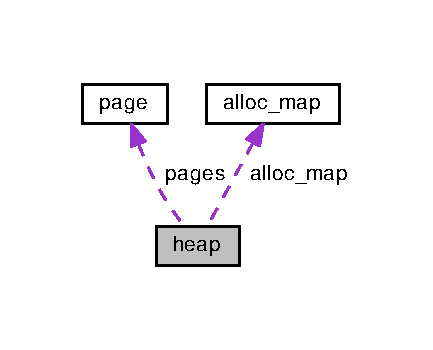
\includegraphics[width=208pt]{structheap__coll__graph}
\end{center}
\end{figure}
\subsection*{Public Attributes}
\begin{DoxyCompactItemize}
\item 
\hypertarget{structheap_aef54d9a3db63859dcfa9a38ebb42823e}{void $\ast$ {\bfseries memory}}\label{structheap_aef54d9a3db63859dcfa9a38ebb42823e}

\item 
\hypertarget{structheap_a01357129b314f4f004b7273869a01ec2}{\hyperlink{alloc__map_8h_a1dd850d0c221c065db145344bbd56714}{alloc\-\_\-map\-\_\-t} $\ast$ {\bfseries alloc\-\_\-map}}\label{structheap_a01357129b314f4f004b7273869a01ec2}

\item 
\hypertarget{structheap_a4c25bc4241337fdea12b53bf8185070d}{size\-\_\-t {\bfseries size}}\label{structheap_a4c25bc4241337fdea12b53bf8185070d}

\item 
\hypertarget{structheap_ac060d2df3b78970d9c23fc1dcec2a921}{bool {\bfseries unsafe\-\_\-stack}}\label{structheap_ac060d2df3b78970d9c23fc1dcec2a921}

\item 
\hypertarget{structheap_aa6580886a3ce54095739d5e07b1bda74}{float {\bfseries gc\-\_\-threshold}}\label{structheap_aa6580886a3ce54095739d5e07b1bda74}

\item 
\hypertarget{structheap_ade55f22f4a2861e9f3a3e3bc6eb32471}{size\-\_\-t {\bfseries number\-\_\-of\-\_\-pages}}\label{structheap_ade55f22f4a2861e9f3a3e3bc6eb32471}

\item 
\hypertarget{structheap_af87be11cb17953345d1ed8034900cadf}{\hyperlink{structpage}{page\-\_\-t} $\ast$ {\bfseries pages} \mbox{[}$\,$\mbox{]}}\label{structheap_af87be11cb17953345d1ed8034900cadf}

\end{DoxyCompactItemize}


The documentation for this struct was generated from the following file\-:\begin{DoxyCompactItemize}
\item 
\hyperlink{gc__hidden_8h}{gc\-\_\-hidden.\-h}\end{DoxyCompactItemize}

\hypertarget{structpage}{}\section{page Struct Reference}
\label{structpage}\index{page@{page}}
\subsection*{Public Attributes}
\begin{DoxyCompactItemize}
\item 
\hypertarget{structpage_a2b3f55e00ff29b84992b5b47f72fb72d}{}void $\ast$ {\bfseries start}\label{structpage_a2b3f55e00ff29b84992b5b47f72fb72d}

\item 
\hypertarget{structpage_a6ad4c9be69d661d94b74fbb7b41f7d3d}{}void $\ast$ {\bfseries bump}\label{structpage_a6ad4c9be69d661d94b74fbb7b41f7d3d}

\item 
\hypertarget{structpage_a077b5c879b7825ab21dad61d96ea9b65}{}size\+\_\+t {\bfseries size}\label{structpage_a077b5c879b7825ab21dad61d96ea9b65}

\item 
\hypertarget{structpage_ab70c0798f1e3ad36842dd8a1454d2b21}{}page\+\_\+type\+\_\+t {\bfseries type}\label{structpage_ab70c0798f1e3ad36842dd8a1454d2b21}

\end{DoxyCompactItemize}


The documentation for this struct was generated from the following file\+:\begin{DoxyCompactItemize}
\item 
\hyperlink{gc__hidden_8h}{gc\+\_\+hidden.\+h}\end{DoxyCompactItemize}

\hypertarget{structtest__link}{\section{test\-\_\-link Struct Reference}
\label{structtest__link}\index{test\-\_\-link@{test\-\_\-link}}
}


Collaboration diagram for test\-\_\-link\-:\nopagebreak
\begin{figure}[H]
\begin{center}
\leavevmode
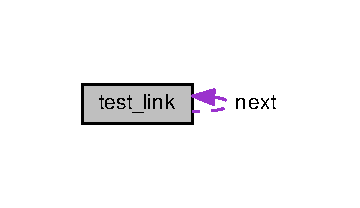
\includegraphics[width=173pt]{structtest__link__coll__graph}
\end{center}
\end{figure}
\subsection*{Public Attributes}
\begin{DoxyCompactItemize}
\item 
\hypertarget{structtest__link_a41da4adc6005519765311723cdd67e4b}{struct \hyperlink{structtest__link}{test\-\_\-link} $\ast$ {\bfseries next}}\label{structtest__link_a41da4adc6005519765311723cdd67e4b}

\item 
\hypertarget{structtest__link_ac632e3031e6095186684a51fa11ab899}{int {\bfseries value}}\label{structtest__link_ac632e3031e6095186684a51fa11ab899}

\end{DoxyCompactItemize}


The documentation for this struct was generated from the following file\-:\begin{DoxyCompactItemize}
\item 
gc\-\_\-test.\-c\end{DoxyCompactItemize}

\hypertarget{structtest__struct}{\section{test\-\_\-struct Struct Reference}
\label{structtest__struct}\index{test\-\_\-struct@{test\-\_\-struct}}
}
\subsection*{Public Attributes}
\begin{DoxyCompactItemize}
\item 
\hypertarget{structtest__struct_af83b58915cfa71e1aecdee37ab6a90e4}{int {\bfseries i}}\label{structtest__struct_af83b58915cfa71e1aecdee37ab6a90e4}

\item 
\hypertarget{structtest__struct_aaa06c5e545861f5e6b24f90b460cc6da}{char {\bfseries c}}\label{structtest__struct_aaa06c5e545861f5e6b24f90b460cc6da}

\item 
\hypertarget{structtest__struct_a54bc6000450b59faa3a791f044ecb8fb}{void $\ast$ {\bfseries ptr}}\label{structtest__struct_a54bc6000450b59faa3a791f044ecb8fb}

\item 
\hypertarget{structtest__struct_a169248f38460a21a2aae898b45fc3107}{long {\bfseries l}}\label{structtest__struct_a169248f38460a21a2aae898b45fc3107}

\item 
\hypertarget{structtest__struct_a74068b2ff3c63ec28ef6686f24133697}{double {\bfseries d}}\label{structtest__struct_a74068b2ff3c63ec28ef6686f24133697}

\end{DoxyCompactItemize}


The documentation for this struct was generated from the following file\-:\begin{DoxyCompactItemize}
\item 
gc\-\_\-test.\-c\end{DoxyCompactItemize}

\chapter{File Documentation}
\hypertarget{alloc__map_8h}{\section{alloc\-\_\-map.\-h File Reference}
\label{alloc__map_8h}\index{alloc\-\_\-map.\-h@{alloc\-\_\-map.\-h}}
}


A module for creating and handling the allocation map. Heavily based on bitmap provided by T. Wrigstad at\-: \href{https://github.com/IOOPM-UU/ioopm16/blob/master/forelasningar/fas1/f12/f12.pdf}{\tt https\-://github.\-com/\-I\-O\-O\-P\-M-\/\-U\-U/ioopm16/blob/master/forelasningar/fas1/f12/f12.\-pdf}.  


{\ttfamily \#include $<$stdbool.\-h$>$}\\*
{\ttfamily \#include $<$stdlib.\-h$>$}\\*
Include dependency graph for alloc\-\_\-map.\-h\-:\nopagebreak
\begin{figure}[H]
\begin{center}
\leavevmode
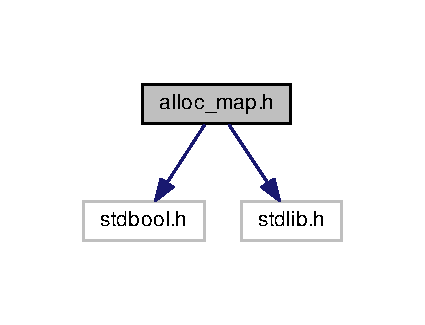
\includegraphics[width=204pt]{alloc__map_8h__incl}
\end{center}
\end{figure}
This graph shows which files directly or indirectly include this file\-:\nopagebreak
\begin{figure}[H]
\begin{center}
\leavevmode
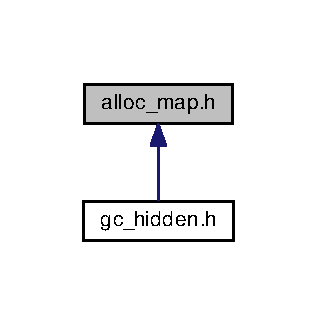
\includegraphics[width=152pt]{alloc__map_8h__dep__incl}
\end{center}
\end{figure}
\subsection*{Typedefs}
\begin{DoxyCompactItemize}
\item 
typedef struct \hyperlink{structalloc__map}{alloc\-\_\-map} \hyperlink{alloc__map_8h_a1dd850d0c221c065db145344bbd56714}{alloc\-\_\-map\-\_\-t}
\end{DoxyCompactItemize}
\subsection*{Functions}
\begin{DoxyCompactItemize}
\item 
void \hyperlink{alloc__map_8h_abd8dc8820178f56815663435082389f4}{alloc\-\_\-map\-\_\-create} (\hyperlink{alloc__map_8h_a1dd850d0c221c065db145344bbd56714}{alloc\-\_\-map\-\_\-t} $\ast$\hyperlink{structalloc__map}{alloc\-\_\-map}, void $\ast$start\-\_\-addr, size\-\_\-t word\-\_\-size, size\-\_\-t block\-\_\-size)
\begin{DoxyCompactList}\small\item\em Creates allocation map. \end{DoxyCompactList}\item 
size\-\_\-t \hyperlink{alloc__map_8h_a9792318f8d96126bd0c5a010a90adfe3}{alloc\-\_\-map\-\_\-mem\-\_\-size\-\_\-needed} (size\-\_\-t word\-\_\-size, size\-\_\-t block\-\_\-size)
\begin{DoxyCompactList}\small\item\em Gets the size needed for an allocation map. \end{DoxyCompactList}\item 
bool \hyperlink{alloc__map_8h_a8a6cb8cdfd0b0fa6f513208adfdfd037}{alloc\-\_\-map\-\_\-ptr\-\_\-used} (\hyperlink{alloc__map_8h_a1dd850d0c221c065db145344bbd56714}{alloc\-\_\-map\-\_\-t} $\ast$\hyperlink{structalloc__map}{alloc\-\_\-map}, void $\ast$ptr)
\begin{DoxyCompactList}\small\item\em Looks up if a memory address is pointing to the start of an object allocated on the gc-\/heap. \end{DoxyCompactList}\item 
bool \hyperlink{alloc__map_8h_a501dcca977bed95d8ff87806cc8a9952}{alloc\-\_\-map\-\_\-set} (\hyperlink{alloc__map_8h_a1dd850d0c221c065db145344bbd56714}{alloc\-\_\-map\-\_\-t} $\ast$\hyperlink{structalloc__map}{alloc\-\_\-map}, void $\ast$ptr, bool state)
\begin{DoxyCompactList}\small\item\em Flags an address. \end{DoxyCompactList}\end{DoxyCompactItemize}


\subsection{Detailed Description}
A module for creating and handling the allocation map. Heavily based on bitmap provided by T. Wrigstad at\-: \href{https://github.com/IOOPM-UU/ioopm16/blob/master/forelasningar/fas1/f12/f12.pdf}{\tt https\-://github.\-com/\-I\-O\-O\-P\-M-\/\-U\-U/ioopm16/blob/master/forelasningar/fas1/f12/f12.\-pdf}. We have discovered that this implementation of allocation map require more memory than what should be needed. Instead of using one bit for each address it need one byte.

\begin{DoxyAuthor}{Author}
Daniel Agstrand 

Henrik Bergendal 

Adam Inersjo 

Maria Lindqvist 

Simon Pellgard 

Robert Rosborg 
\end{DoxyAuthor}


\subsection{Typedef Documentation}
\hypertarget{alloc__map_8h_a1dd850d0c221c065db145344bbd56714}{\index{alloc\-\_\-map.\-h@{alloc\-\_\-map.\-h}!alloc\-\_\-map\-\_\-t@{alloc\-\_\-map\-\_\-t}}
\index{alloc\-\_\-map\-\_\-t@{alloc\-\_\-map\-\_\-t}!alloc_map.h@{alloc\-\_\-map.\-h}}
\subsubsection[{alloc\-\_\-map\-\_\-t}]{\setlength{\rightskip}{0pt plus 5cm}typedef struct {\bf alloc\-\_\-map} {\bf alloc\-\_\-map\-\_\-t}}}\label{alloc__map_8h_a1dd850d0c221c065db145344bbd56714}
The alloc map is a collection of boolean values each showing if an adress on the heap is at the start of an object. 

\subsection{Function Documentation}
\hypertarget{alloc__map_8h_abd8dc8820178f56815663435082389f4}{\index{alloc\-\_\-map.\-h@{alloc\-\_\-map.\-h}!alloc\-\_\-map\-\_\-create@{alloc\-\_\-map\-\_\-create}}
\index{alloc\-\_\-map\-\_\-create@{alloc\-\_\-map\-\_\-create}!alloc_map.h@{alloc\-\_\-map.\-h}}
\subsubsection[{alloc\-\_\-map\-\_\-create}]{\setlength{\rightskip}{0pt plus 5cm}void alloc\-\_\-map\-\_\-create (
\begin{DoxyParamCaption}
\item[{{\bf alloc\-\_\-map\-\_\-t} $\ast$}]{alloc\-\_\-map, }
\item[{void $\ast$}]{start\-\_\-addr, }
\item[{size\-\_\-t}]{word\-\_\-size, }
\item[{size\-\_\-t}]{block\-\_\-size}
\end{DoxyParamCaption}
)}}\label{alloc__map_8h_abd8dc8820178f56815663435082389f4}


Creates allocation map. 

This function creates an allocation map on the provided pointer.


\begin{DoxyParams}{Parameters}
{\em \hyperlink{structalloc__map}{alloc\-\_\-map}} & the adress where the allocation map is to be created.\\
\hline
{\em start\-\_\-addr} & the starting address for the memory block the allocation map represents. \\
\hline
{\em word\-\_\-size} & the size of the words which the memory block is divided into. \\
\hline
{\em block\-\_\-size} & the size in bytes of the memory block the map is going to represent \\
\hline
\end{DoxyParams}
\hypertarget{alloc__map_8h_a9792318f8d96126bd0c5a010a90adfe3}{\index{alloc\-\_\-map.\-h@{alloc\-\_\-map.\-h}!alloc\-\_\-map\-\_\-mem\-\_\-size\-\_\-needed@{alloc\-\_\-map\-\_\-mem\-\_\-size\-\_\-needed}}
\index{alloc\-\_\-map\-\_\-mem\-\_\-size\-\_\-needed@{alloc\-\_\-map\-\_\-mem\-\_\-size\-\_\-needed}!alloc_map.h@{alloc\-\_\-map.\-h}}
\subsubsection[{alloc\-\_\-map\-\_\-mem\-\_\-size\-\_\-needed}]{\setlength{\rightskip}{0pt plus 5cm}size\-\_\-t alloc\-\_\-map\-\_\-mem\-\_\-size\-\_\-needed (
\begin{DoxyParamCaption}
\item[{size\-\_\-t}]{word\-\_\-size, }
\item[{size\-\_\-t}]{block\-\_\-size}
\end{DoxyParamCaption}
)}}\label{alloc__map_8h_a9792318f8d96126bd0c5a010a90adfe3}


Gets the size needed for an allocation map. 


\begin{DoxyParams}{Parameters}
{\em word\-\_\-size} & the size of the words which the memory block is divided into.\\
\hline
{\em block\-\_\-size} & the size in bytes of the memory block the map is going to represent.\\
\hline
\end{DoxyParams}
\begin{DoxyReturn}{Returns}
the size in bytes needed to store the allocation map. 
\end{DoxyReturn}
\hypertarget{alloc__map_8h_a8a6cb8cdfd0b0fa6f513208adfdfd037}{\index{alloc\-\_\-map.\-h@{alloc\-\_\-map.\-h}!alloc\-\_\-map\-\_\-ptr\-\_\-used@{alloc\-\_\-map\-\_\-ptr\-\_\-used}}
\index{alloc\-\_\-map\-\_\-ptr\-\_\-used@{alloc\-\_\-map\-\_\-ptr\-\_\-used}!alloc_map.h@{alloc\-\_\-map.\-h}}
\subsubsection[{alloc\-\_\-map\-\_\-ptr\-\_\-used}]{\setlength{\rightskip}{0pt plus 5cm}bool alloc\-\_\-map\-\_\-ptr\-\_\-used (
\begin{DoxyParamCaption}
\item[{{\bf alloc\-\_\-map\-\_\-t} $\ast$}]{alloc\-\_\-map, }
\item[{void $\ast$}]{ptr}
\end{DoxyParamCaption}
)}}\label{alloc__map_8h_a8a6cb8cdfd0b0fa6f513208adfdfd037}


Looks up if a memory address is pointing to the start of an object allocated on the gc-\/heap. 


\begin{DoxyParams}{Parameters}
{\em \hyperlink{structalloc__map}{alloc\-\_\-map}} & pointer to the alloc map. \\
\hline
{\em ptr} & pointer to the adress to look up.\\
\hline
\end{DoxyParams}
\begin{DoxyReturn}{Returns}
A bool representing the bit of the supplied ptr. False if {\ttfamily ptr} not in scope of {\ttfamily \hyperlink{structalloc__map}{alloc\-\_\-map}} 
\end{DoxyReturn}
\hypertarget{alloc__map_8h_a501dcca977bed95d8ff87806cc8a9952}{\index{alloc\-\_\-map.\-h@{alloc\-\_\-map.\-h}!alloc\-\_\-map\-\_\-set@{alloc\-\_\-map\-\_\-set}}
\index{alloc\-\_\-map\-\_\-set@{alloc\-\_\-map\-\_\-set}!alloc_map.h@{alloc\-\_\-map.\-h}}
\subsubsection[{alloc\-\_\-map\-\_\-set}]{\setlength{\rightskip}{0pt plus 5cm}bool alloc\-\_\-map\-\_\-set (
\begin{DoxyParamCaption}
\item[{{\bf alloc\-\_\-map\-\_\-t} $\ast$}]{alloc\-\_\-map, }
\item[{void $\ast$}]{ptr, }
\item[{bool}]{state}
\end{DoxyParamCaption}
)}}\label{alloc__map_8h_a501dcca977bed95d8ff87806cc8a9952}


Flags an address. 


\begin{DoxyParams}{Parameters}
{\em \hyperlink{structalloc__map}{alloc\-\_\-map}} & pointer to the alloc map \\
\hline
{\em ptr} & the pointer to set. \\
\hline
{\em state} & the value to set. \\
\hline
\end{DoxyParams}

\hypertarget{gc_8h}{}\section{gc.\+h File Reference}
\label{gc_8h}\index{gc.\+h@{gc.\+h}}


A library for heap allocation with automatic garbage collection.  


{\ttfamily \#include $<$stdbool.\+h$>$}\\*
{\ttfamily \#include $<$stdint.\+h$>$}\\*
{\ttfamily \#include $<$stdlib.\+h$>$}\\*
Include dependency graph for gc.\+h\+:
% FIG 0
This graph shows which files directly or indirectly include this file\+:
% FIG 1
\subsection*{Macros}
\begin{DoxyCompactItemize}
\item 
\hypertarget{gc_8h_a0f4834f5dfa7df354e5bfd36528ee4d6}{}\#define {\bfseries U\+N\+S\+A\+F\+E\+\_\+\+S\+T\+A\+C\+K}~true\label{gc_8h_a0f4834f5dfa7df354e5bfd36528ee4d6}

\item 
\hypertarget{gc_8h_a2582f8409ae69733c2471793710c23ea}{}\#define {\bfseries S\+A\+F\+E\+\_\+\+S\+T\+A\+C\+K}~false\label{gc_8h_a2582f8409ae69733c2471793710c23ea}

\end{DoxyCompactItemize}
\subsection*{Typedefs}
\begin{DoxyCompactItemize}
\item 
\hypertarget{gc_8h_ad3bb09826584eab4757c6cd2f988e7d6}{}typedef struct \hyperlink{structheap}{heap} \hyperlink{gc_8h_ad3bb09826584eab4757c6cd2f988e7d6}{heap\+\_\+t}\label{gc_8h_ad3bb09826584eab4757c6cd2f988e7d6}

\begin{DoxyCompactList}\small\item\em The opaque data type holding all the heap data. \end{DoxyCompactList}\end{DoxyCompactItemize}
\subsection*{Functions}
\begin{DoxyCompactItemize}
\item 
\hyperlink{gc_8h_ad3bb09826584eab4757c6cd2f988e7d6}{heap\+\_\+t} $\ast$ \hyperlink{gc_8h_ab63ddbc8bdc711c2879417b0faafe530}{h\+\_\+init} (size\+\_\+t bytes, bool unsafe\+\_\+stack, float gc\+\_\+threshold)
\begin{DoxyCompactList}\small\item\em Create a new heap with {\ttfamily bytes} total size. \end{DoxyCompactList}\item 
void \hyperlink{gc_8h_a2a33b69784524edff57993a64c1c6616}{h\+\_\+delete} (\hyperlink{gc_8h_ad3bb09826584eab4757c6cd2f988e7d6}{heap\+\_\+t} $\ast$h)
\begin{DoxyCompactList}\small\item\em Delete a heap. \end{DoxyCompactList}\item 
void \hyperlink{gc_8h_aee911cf9474117bcbb06c53aed4f9288}{h\+\_\+delete\+\_\+dbg} (\hyperlink{gc_8h_ad3bb09826584eab4757c6cd2f988e7d6}{heap\+\_\+t} $\ast$h, void $\ast$dbg\+\_\+value)
\begin{DoxyCompactList}\small\item\em Delete a heap and trace, killing off stack pointers. \end{DoxyCompactList}\item 
void $\ast$ \hyperlink{gc_8h_afc09bd012e52f4e533e798077e2bfd6d}{h\+\_\+alloc\+\_\+struct} (\hyperlink{gc_8h_ad3bb09826584eab4757c6cd2f988e7d6}{heap\+\_\+t} $\ast$h, char $\ast$layout)
\begin{DoxyCompactList}\small\item\em Allocate a new object on a heap with a given format string. \end{DoxyCompactList}\item 
void $\ast$ \hyperlink{gc_8h_a7135f8d1dfd9ce92bec0db717334c0ee}{h\+\_\+alloc\+\_\+data} (\hyperlink{gc_8h_ad3bb09826584eab4757c6cd2f988e7d6}{heap\+\_\+t} $\ast$h, size\+\_\+t bytes)
\begin{DoxyCompactList}\small\item\em Allocate a new object on a heap with a given size. \end{DoxyCompactList}\item 
size\+\_\+t \hyperlink{gc_8h_ad7dc4368eb1d50f161d20c18d83d5610}{h\+\_\+gc} (\hyperlink{gc_8h_ad3bb09826584eab4757c6cd2f988e7d6}{heap\+\_\+t} $\ast$h)
\begin{DoxyCompactList}\small\item\em Manually trigger garbage collection. \end{DoxyCompactList}\item 
size\+\_\+t \hyperlink{gc_8h_a348b1f7af1f7cbe8ba83820fe503a0b4}{h\+\_\+gc\+\_\+dbg} (\hyperlink{gc_8h_ad3bb09826584eab4757c6cd2f988e7d6}{heap\+\_\+t} $\ast$h, bool unsafe\+\_\+stack)
\begin{DoxyCompactList}\small\item\em Manually trigger garbage collection with the ability to override the setting for how stack pointers are treated. \end{DoxyCompactList}\item 
size\+\_\+t \hyperlink{gc_8h_ae5a02e78fb87061975e8b509375d7eb8}{h\+\_\+avail} (\hyperlink{gc_8h_ad3bb09826584eab4757c6cd2f988e7d6}{heap\+\_\+t} $\ast$h)
\begin{DoxyCompactList}\small\item\em Returns the available free memory. \end{DoxyCompactList}\item 
size\+\_\+t \hyperlink{gc_8h_adf4518289fe36bdd40c5e80362063fd4}{h\+\_\+used} (\hyperlink{gc_8h_ad3bb09826584eab4757c6cd2f988e7d6}{heap\+\_\+t} $\ast$h)
\begin{DoxyCompactList}\small\item\em Returns the bytes currently in use in a heap. \end{DoxyCompactList}\item 
size\+\_\+t \hyperlink{gc_8h_ab6dea3c2f2058c8dd2d172a109634fec}{h\+\_\+size} (\hyperlink{gc_8h_ad3bb09826584eab4757c6cd2f988e7d6}{heap\+\_\+t} $\ast$h)
\begin{DoxyCompactList}\small\item\em Return the byte size of the heap. \end{DoxyCompactList}\item 
char $\ast$ \hyperlink{gc_8h_abf464a743697b9f7c3e913be239e9f9d}{h\+\_\+strdup} (\hyperlink{gc_8h_ad3bb09826584eab4757c6cd2f988e7d6}{heap\+\_\+t} $\ast$h, char $\ast$str)
\begin{DoxyCompactList}\small\item\em Return a copy of a pointer, that is alloced on our heap. $\ast$. \end{DoxyCompactList}\end{DoxyCompactItemize}


\subsection{Detailed Description}
A library for heap allocation with automatic garbage collection. 

\begin{DoxyAuthor}{Author}
Daniel Agstrand 

Henrik Bergendal 

Adam Inersjo 

Maria Lindqvist 

Simon Pellgard 

Robert Rosborg 
\end{DoxyAuthor}


\subsection{Function Documentation}
\hypertarget{gc_8h_a7135f8d1dfd9ce92bec0db717334c0ee}{}\index{gc.\+h@{gc.\+h}!h\+\_\+alloc\+\_\+data@{h\+\_\+alloc\+\_\+data}}
\index{h\+\_\+alloc\+\_\+data@{h\+\_\+alloc\+\_\+data}!gc.\+h@{gc.\+h}}
\subsubsection[{h\+\_\+alloc\+\_\+data}]{\setlength{\rightskip}{0pt plus 5cm}void$\ast$ h\+\_\+alloc\+\_\+data (
\begin{DoxyParamCaption}
\item[{{\bf heap\+\_\+t} $\ast$}]{h, }
\item[{size\+\_\+t}]{bytes}
\end{DoxyParamCaption}
)}\label{gc_8h_a7135f8d1dfd9ce92bec0db717334c0ee}


Allocate a new object on a heap with a given size. 

Objects allocated with this function will {\itshape not} be further traced for pointers.


\begin{DoxyParams}{Parameters}
{\em h} & the heap \\
\hline
{\em bytes} & the size in bytes \\
\hline
\end{DoxyParams}
\begin{DoxyReturn}{Returns}
the newly allocated object 
\end{DoxyReturn}
\hypertarget{gc_8h_afc09bd012e52f4e533e798077e2bfd6d}{}\index{gc.\+h@{gc.\+h}!h\+\_\+alloc\+\_\+struct@{h\+\_\+alloc\+\_\+struct}}
\index{h\+\_\+alloc\+\_\+struct@{h\+\_\+alloc\+\_\+struct}!gc.\+h@{gc.\+h}}
\subsubsection[{h\+\_\+alloc\+\_\+struct}]{\setlength{\rightskip}{0pt plus 5cm}void$\ast$ h\+\_\+alloc\+\_\+struct (
\begin{DoxyParamCaption}
\item[{{\bf heap\+\_\+t} $\ast$}]{h, }
\item[{char $\ast$}]{layout}
\end{DoxyParamCaption}
)}\label{gc_8h_afc09bd012e52f4e533e798077e2bfd6d}


Allocate a new object on a heap with a given format string. 

Valid characters in format strings are\+:
\begin{DoxyItemize}
\item \textquotesingle{}i\textquotesingle{} -- for sizeof(int) bytes \textquotesingle{}raw\textquotesingle{} data
\item \textquotesingle{}l\textquotesingle{} -- for sizeof(long) bytes \textquotesingle{}raw\textquotesingle{} data
\item \textquotesingle{}f\textquotesingle{} -- for sizeof(float) bytes \textquotesingle{}raw\textquotesingle{} data
\item \textquotesingle{}c\textquotesingle{} -- for sizeof(char) bytes \textquotesingle{}raw\textquotesingle{} data
\item \textquotesingle{}d\textquotesingle{} -- for sizeof(double) bytes \textquotesingle{}raw\textquotesingle{} data
\item \textquotesingle{}$\ast$\textquotesingle{} -- for a sizeof(void $\ast$) bytes pointer value
\item \textquotesingle{}\textbackslash{}0\textquotesingle{} -- null-\/character terminates the format string
\end{DoxyItemize}


\begin{DoxyParams}{Parameters}
{\em h} & the heap \\
\hline
{\em layout} & the format string \\
\hline
\end{DoxyParams}
\begin{DoxyReturn}{Returns}
the newly allocated object
\end{DoxyReturn}
\begin{DoxyNote}{Note}
the heap does {\itshape not} retain an alias to layout. 
\end{DoxyNote}
\hypertarget{gc_8h_ae5a02e78fb87061975e8b509375d7eb8}{}\index{gc.\+h@{gc.\+h}!h\+\_\+avail@{h\+\_\+avail}}
\index{h\+\_\+avail@{h\+\_\+avail}!gc.\+h@{gc.\+h}}
\subsubsection[{h\+\_\+avail}]{\setlength{\rightskip}{0pt plus 5cm}size\+\_\+t h\+\_\+avail (
\begin{DoxyParamCaption}
\item[{{\bf heap\+\_\+t} $\ast$}]{h}
\end{DoxyParamCaption}
)}\label{gc_8h_ae5a02e78fb87061975e8b509375d7eb8}


Returns the available free memory. 


\begin{DoxyParams}{Parameters}
{\em h} & the heap \\
\hline
\end{DoxyParams}
\begin{DoxyReturn}{Returns}
the available free memory. 
\end{DoxyReturn}
\hypertarget{gc_8h_a2a33b69784524edff57993a64c1c6616}{}\index{gc.\+h@{gc.\+h}!h\+\_\+delete@{h\+\_\+delete}}
\index{h\+\_\+delete@{h\+\_\+delete}!gc.\+h@{gc.\+h}}
\subsubsection[{h\+\_\+delete}]{\setlength{\rightskip}{0pt plus 5cm}void h\+\_\+delete (
\begin{DoxyParamCaption}
\item[{{\bf heap\+\_\+t} $\ast$}]{h}
\end{DoxyParamCaption}
)}\label{gc_8h_a2a33b69784524edff57993a64c1c6616}


Delete a heap. 


\begin{DoxyParams}{Parameters}
{\em h} & the heap \\
\hline
\end{DoxyParams}
\hypertarget{gc_8h_aee911cf9474117bcbb06c53aed4f9288}{}\index{gc.\+h@{gc.\+h}!h\+\_\+delete\+\_\+dbg@{h\+\_\+delete\+\_\+dbg}}
\index{h\+\_\+delete\+\_\+dbg@{h\+\_\+delete\+\_\+dbg}!gc.\+h@{gc.\+h}}
\subsubsection[{h\+\_\+delete\+\_\+dbg}]{\setlength{\rightskip}{0pt plus 5cm}void h\+\_\+delete\+\_\+dbg (
\begin{DoxyParamCaption}
\item[{{\bf heap\+\_\+t} $\ast$}]{h, }
\item[{void $\ast$}]{dbg\+\_\+value}
\end{DoxyParamCaption}
)}\label{gc_8h_aee911cf9474117bcbb06c53aed4f9288}


Delete a heap and trace, killing off stack pointers. 

Only valid pointers will be replaced. A valid pointer is a pointer with the address of an allocated space in {\ttfamily h}.


\begin{DoxyParams}{Parameters}
{\em h} & the heap \\
\hline
{\em dbg\+\_\+value} & a value to be written into every valid pointer into {\ttfamily h} on the stack \\
\hline
\end{DoxyParams}
\hypertarget{gc_8h_ad7dc4368eb1d50f161d20c18d83d5610}{}\index{gc.\+h@{gc.\+h}!h\+\_\+gc@{h\+\_\+gc}}
\index{h\+\_\+gc@{h\+\_\+gc}!gc.\+h@{gc.\+h}}
\subsubsection[{h\+\_\+gc}]{\setlength{\rightskip}{0pt plus 5cm}size\+\_\+t h\+\_\+gc (
\begin{DoxyParamCaption}
\item[{{\bf heap\+\_\+t} $\ast$}]{h}
\end{DoxyParamCaption}
)}\label{gc_8h_ad7dc4368eb1d50f161d20c18d83d5610}


Manually trigger garbage collection. 

Garbage collection is otherwise run when an allocation is impossible in the available consecutive free memory.


\begin{DoxyParams}{Parameters}
{\em h} & the heap \\
\hline
\end{DoxyParams}
\begin{DoxyReturn}{Returns}
the number of bytes collected 
\end{DoxyReturn}
\hypertarget{gc_8h_a348b1f7af1f7cbe8ba83820fe503a0b4}{}\index{gc.\+h@{gc.\+h}!h\+\_\+gc\+\_\+dbg@{h\+\_\+gc\+\_\+dbg}}
\index{h\+\_\+gc\+\_\+dbg@{h\+\_\+gc\+\_\+dbg}!gc.\+h@{gc.\+h}}
\subsubsection[{h\+\_\+gc\+\_\+dbg}]{\setlength{\rightskip}{0pt plus 5cm}size\+\_\+t h\+\_\+gc\+\_\+dbg (
\begin{DoxyParamCaption}
\item[{{\bf heap\+\_\+t} $\ast$}]{h, }
\item[{bool}]{unsafe\+\_\+stack}
\end{DoxyParamCaption}
)}\label{gc_8h_a348b1f7af1f7cbe8ba83820fe503a0b4}


Manually trigger garbage collection with the ability to override the setting for how stack pointers are treated. 

Garbage collection is otherwise run when an allocation is impossible in the available consecutive free memory.


\begin{DoxyParams}{Parameters}
{\em h} & the heap \\
\hline
{\em unsafe\+\_\+stack} & true if pointers on the stack are to be considered unsafe pointers \\
\hline
\end{DoxyParams}
\begin{DoxyReturn}{Returns}
the number of bytes collected 
\end{DoxyReturn}
\hypertarget{gc_8h_ab63ddbc8bdc711c2879417b0faafe530}{}\index{gc.\+h@{gc.\+h}!h\+\_\+init@{h\+\_\+init}}
\index{h\+\_\+init@{h\+\_\+init}!gc.\+h@{gc.\+h}}
\subsubsection[{h\+\_\+init}]{\setlength{\rightskip}{0pt plus 5cm}{\bf heap\+\_\+t}$\ast$ h\+\_\+init (
\begin{DoxyParamCaption}
\item[{size\+\_\+t}]{bytes, }
\item[{bool}]{unsafe\+\_\+stack, }
\item[{float}]{gc\+\_\+threshold}
\end{DoxyParamCaption}
)}\label{gc_8h_ab63ddbc8bdc711c2879417b0faafe530}


Create a new heap with {\ttfamily bytes} total size. 

The size available for allocation will be strictly less than {\ttfamily bytes} because of metadata and other internal data.


\begin{DoxyParams}{Parameters}
{\em bytes} & the total size of the heap in bytes \\
\hline
{\em unsafe\+\_\+stack} & true if pointers on the stack are to be considered unsafe pointers \\
\hline
{\em gc\+\_\+threshold} & the memory pressure at which gc should be triggered (1.\+0 = full memory) \\
\hline
\end{DoxyParams}
\begin{DoxyReturn}{Returns}
the new heap or N\+U\+L\+L if memory cannot be allocated 
\end{DoxyReturn}
\hypertarget{gc_8h_ab6dea3c2f2058c8dd2d172a109634fec}{}\index{gc.\+h@{gc.\+h}!h\+\_\+size@{h\+\_\+size}}
\index{h\+\_\+size@{h\+\_\+size}!gc.\+h@{gc.\+h}}
\subsubsection[{h\+\_\+size}]{\setlength{\rightskip}{0pt plus 5cm}size\+\_\+t h\+\_\+size (
\begin{DoxyParamCaption}
\item[{{\bf heap\+\_\+t} $\ast$}]{h}
\end{DoxyParamCaption}
)}\label{gc_8h_ab6dea3c2f2058c8dd2d172a109634fec}


Return the byte size of the heap. 


\begin{DoxyParams}{Parameters}
{\em h} & the heap \\
\hline
\end{DoxyParams}
\begin{DoxyReturn}{Returns}
the byte size of the heap. 
\end{DoxyReturn}
\hypertarget{gc_8h_abf464a743697b9f7c3e913be239e9f9d}{}\index{gc.\+h@{gc.\+h}!h\+\_\+strdup@{h\+\_\+strdup}}
\index{h\+\_\+strdup@{h\+\_\+strdup}!gc.\+h@{gc.\+h}}
\subsubsection[{h\+\_\+strdup}]{\setlength{\rightskip}{0pt plus 5cm}char$\ast$ h\+\_\+strdup (
\begin{DoxyParamCaption}
\item[{{\bf heap\+\_\+t} $\ast$}]{h, }
\item[{char $\ast$}]{str}
\end{DoxyParamCaption}
)}\label{gc_8h_abf464a743697b9f7c3e913be239e9f9d}


Return a copy of a pointer, that is alloced on our heap. $\ast$. 


\begin{DoxyParams}{Parameters}
{\em h} & the heap \\
\hline
{\em str} & the pointer to the string \\
\hline
\end{DoxyParams}
\begin{DoxyReturn}{Returns}
The copied pointer 
\end{DoxyReturn}
\hypertarget{gc_8h_adf4518289fe36bdd40c5e80362063fd4}{}\index{gc.\+h@{gc.\+h}!h\+\_\+used@{h\+\_\+used}}
\index{h\+\_\+used@{h\+\_\+used}!gc.\+h@{gc.\+h}}
\subsubsection[{h\+\_\+used}]{\setlength{\rightskip}{0pt plus 5cm}size\+\_\+t h\+\_\+used (
\begin{DoxyParamCaption}
\item[{{\bf heap\+\_\+t} $\ast$}]{h}
\end{DoxyParamCaption}
)}\label{gc_8h_adf4518289fe36bdd40c5e80362063fd4}


Returns the bytes currently in use in a heap. 

This includes any meta-\/data specific to user allocated structures and any internal padding.


\begin{DoxyParams}{Parameters}
{\em h} & the heap \\
\hline
\end{DoxyParams}
\begin{DoxyReturn}{Returns}
the bytes currently in use by user structures. 
\end{DoxyReturn}

\hypertarget{gc__hidden_8h}{\section{gc\-\_\-hidden.\-h File Reference}
\label{gc__hidden_8h}\index{gc\-\_\-hidden.\-h@{gc\-\_\-hidden.\-h}}
}


Hidden library for gc.  


{\ttfamily \#include $<$stdbool.\-h$>$}\\*
{\ttfamily \#include $<$stdint.\-h$>$}\\*
{\ttfamily \#include $<$stdlib.\-h$>$}\\*
{\ttfamily \#include \char`\"{}gc.\-h\char`\"{}}\\*
{\ttfamily \#include \char`\"{}alloc\-\_\-map.\-h\char`\"{}}\\*
Include dependency graph for gc\-\_\-hidden.\-h\-:\nopagebreak
\begin{figure}[H]
\begin{center}
\leavevmode
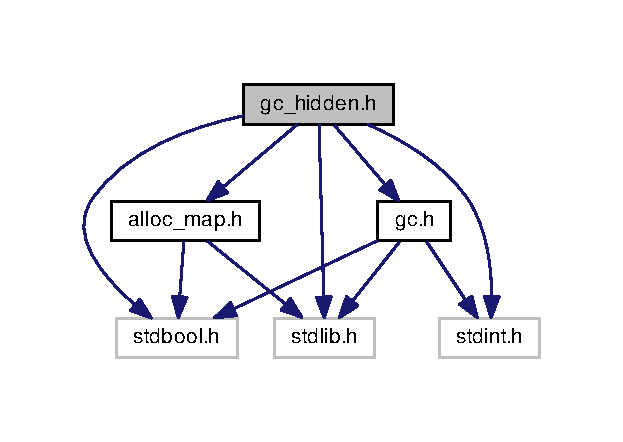
\includegraphics[width=299pt]{gc__hidden_8h__incl}
\end{center}
\end{figure}
\subsection*{Classes}
\begin{DoxyCompactItemize}
\item 
struct \hyperlink{structpage}{page}
\item 
struct \hyperlink{structheap}{heap}
\end{DoxyCompactItemize}
\subsection*{Typedefs}
\begin{DoxyCompactItemize}
\item 
\hypertarget{gc__hidden_8h_ade89166d54350940b6a08604d1119f4e}{typedef struct \hyperlink{structpage}{page} {\bfseries page\-\_\-t}}\label{gc__hidden_8h_ade89166d54350940b6a08604d1119f4e}

\item 
\hypertarget{gc__hidden_8h_a8c49f07bc20bf69652f53495851b4742}{typedef enum page\-\_\-type {\bfseries page\-\_\-type\-\_\-t}}\label{gc__hidden_8h_a8c49f07bc20bf69652f53495851b4742}

\end{DoxyCompactItemize}
\subsection*{Enumerations}
\begin{DoxyCompactItemize}
\item 
enum {\bfseries page\-\_\-type} \{ {\bfseries P\-A\-S\-S\-I\-V\-E}, 
{\bfseries A\-C\-T\-I\-V\-E}, 
{\bfseries T\-R\-A\-N\-S\-I\-T\-I\-O\-N}, 
{\bfseries U\-N\-S\-A\-F\-E}
 \}
\end{DoxyCompactItemize}
\subsection*{Functions}
\begin{DoxyCompactItemize}
\item 
\hypertarget{gc__hidden_8h_a781abd7be7d7a5323f646dad56732c8b}{void $\ast$ {\bfseries get\-\_\-page\-\_\-start} (\hyperlink{structpage}{page\-\_\-t} $\ast$\hyperlink{structpage}{page})}\label{gc__hidden_8h_a781abd7be7d7a5323f646dad56732c8b}

\item 
\hypertarget{gc__hidden_8h_aa8e5e7bdea00913e5dc5cb4e45c3e4d5}{int {\bfseries get\-\_\-ptr\-\_\-page} (\hyperlink{gc_8h_ad3bb09826584eab4757c6cd2f988e7d6}{heap\-\_\-t} $\ast$h, void $\ast$ptr)}\label{gc__hidden_8h_aa8e5e7bdea00913e5dc5cb4e45c3e4d5}

\item 
\hypertarget{gc__hidden_8h_afabf58bea4d81eb1806f0106c38d72ca}{size\-\_\-t {\bfseries page\-\_\-get\-\_\-used} (\hyperlink{structpage}{page\-\_\-t} $\ast$p)}\label{gc__hidden_8h_afabf58bea4d81eb1806f0106c38d72ca}

\item 
\hypertarget{gc__hidden_8h_a1d142dc8aa5e1041d387ac2923c02685}{void $\ast$ {\bfseries get\-\_\-memory} (\hyperlink{gc_8h_ad3bb09826584eab4757c6cd2f988e7d6}{heap\-\_\-t} $\ast$h)}\label{gc__hidden_8h_a1d142dc8aa5e1041d387ac2923c02685}

\item 
\hypertarget{gc__hidden_8h_ac6ceee057a341916a64ee5ba0c0d0cbe}{size\-\_\-t {\bfseries heap\-\_\-get\-\_\-size} (\hyperlink{gc_8h_ad3bb09826584eab4757c6cd2f988e7d6}{heap\-\_\-t} $\ast$h)}\label{gc__hidden_8h_ac6ceee057a341916a64ee5ba0c0d0cbe}

\item 
\hypertarget{gc__hidden_8h_a3721ce5ae94312990e1af97c560d1509}{size\-\_\-t {\bfseries heap\-\_\-get\-\_\-number\-\_\-of\-\_\-pages} (\hyperlink{gc_8h_ad3bb09826584eab4757c6cd2f988e7d6}{heap\-\_\-t} $\ast$h)}\label{gc__hidden_8h_a3721ce5ae94312990e1af97c560d1509}

\item 
\hypertarget{gc__hidden_8h_a9897047994747c4a4aa6583223f98813}{void $\ast$ {\bfseries get\-\_\-stack\-\_\-top} ()}\label{gc__hidden_8h_a9897047994747c4a4aa6583223f98813}

\item 
size\-\_\-t \hyperlink{gc__hidden_8h_a925ef1d5efea33785f11faddf4ee187e}{get\-\_\-number\-\_\-of\-\_\-ptrs\-\_\-in\-\_\-stack} (\hyperlink{gc_8h_ad3bb09826584eab4757c6cd2f988e7d6}{heap\-\_\-t} $\ast$h, void $\ast$original\-\_\-top)
\begin{DoxyCompactList}\small\item\em Gets the number of pointer found on stack. \end{DoxyCompactList}\item 
size\-\_\-t \hyperlink{gc__hidden_8h_a460644011187cc598465fd8ad68c38a2}{get\-\_\-ptrs\-\_\-from\-\_\-stack} (\hyperlink{gc_8h_ad3bb09826584eab4757c6cd2f988e7d6}{heap\-\_\-t} $\ast$h, void $\ast$original\-\_\-top, void $\ast$$\ast$array\mbox{[}$\,$\mbox{]}, size\-\_\-t array\-\_\-size)
\begin{DoxyCompactList}\small\item\em Puts the pointers found on the stack in an array. \end{DoxyCompactList}\item 
size\-\_\-t \hyperlink{gc__hidden_8h_a54614e4098b51e0cd63ecd469647081e}{get\-\_\-number\-\_\-of\-\_\-active\-\_\-ptrs} (\hyperlink{gc_8h_ad3bb09826584eab4757c6cd2f988e7d6}{heap\-\_\-t} $\ast$h, void $\ast$original\-\_\-top)
\begin{DoxyCompactList}\small\item\em Gets the number of active pointers on the stack and in the heap. \end{DoxyCompactList}\item 
size\-\_\-t \hyperlink{gc__hidden_8h_ab1a84d360233bebc46f6a269973e524e}{get\-\_\-active\-\_\-ptrs} (\hyperlink{gc_8h_ad3bb09826584eab4757c6cd2f988e7d6}{heap\-\_\-t} $\ast$h, void $\ast$original\-\_\-top, void $\ast$$\ast$array\mbox{[}$\,$\mbox{]}, size\-\_\-t array\-\_\-size)
\begin{DoxyCompactList}\small\item\em Gets all the active pointers on the stack and in the heap and puts them into an array. \end{DoxyCompactList}\end{DoxyCompactItemize}
\subsection*{Variables}
\begin{DoxyCompactItemize}
\item 
\hypertarget{gc__hidden_8h_aa006daaf11f1e2e45a6ababaf463212b}{char $\ast$$\ast$ {\bfseries environ}}\label{gc__hidden_8h_aa006daaf11f1e2e45a6ababaf463212b}

\end{DoxyCompactItemize}


\subsection{Detailed Description}
Hidden library for gc. \begin{DoxyAuthor}{Author}
Daniel Agstrand 

Henrik Bergendal 

Adam Inersjo 

Maria Lindqvist 

Simon Pellgard 

Robert Rosborg 
\end{DoxyAuthor}


\subsection{Function Documentation}
\hypertarget{gc__hidden_8h_ab1a84d360233bebc46f6a269973e524e}{\index{gc\-\_\-hidden.\-h@{gc\-\_\-hidden.\-h}!get\-\_\-active\-\_\-ptrs@{get\-\_\-active\-\_\-ptrs}}
\index{get\-\_\-active\-\_\-ptrs@{get\-\_\-active\-\_\-ptrs}!gc_hidden.h@{gc\-\_\-hidden.\-h}}
\subsubsection[{get\-\_\-active\-\_\-ptrs}]{\setlength{\rightskip}{0pt plus 5cm}size\-\_\-t get\-\_\-active\-\_\-ptrs (
\begin{DoxyParamCaption}
\item[{{\bf heap\-\_\-t} $\ast$}]{h, }
\item[{void $\ast$}]{original\-\_\-top, }
\item[{void $\ast$$\ast$}]{array\mbox{[}$\,$\mbox{]}, }
\item[{size\-\_\-t}]{array\-\_\-size}
\end{DoxyParamCaption}
)}}\label{gc__hidden_8h_ab1a84d360233bebc46f6a269973e524e}


Gets all the active pointers on the stack and in the heap and puts them into an array. 


\begin{DoxyParams}{Parameters}
{\em h} & a pointer to the heap \\
\hline
{\em original\-\_\-top} & the top of the stack to search \\
\hline
{\em array} & an array of double pointers \\
\hline
{\em array\-\_\-size} & the size of the array\\
\hline
\end{DoxyParams}
\begin{DoxyReturn}{Returns}
the number of pointer found on stack and the heap 
\end{DoxyReturn}
\hypertarget{gc__hidden_8h_a54614e4098b51e0cd63ecd469647081e}{\index{gc\-\_\-hidden.\-h@{gc\-\_\-hidden.\-h}!get\-\_\-number\-\_\-of\-\_\-active\-\_\-ptrs@{get\-\_\-number\-\_\-of\-\_\-active\-\_\-ptrs}}
\index{get\-\_\-number\-\_\-of\-\_\-active\-\_\-ptrs@{get\-\_\-number\-\_\-of\-\_\-active\-\_\-ptrs}!gc_hidden.h@{gc\-\_\-hidden.\-h}}
\subsubsection[{get\-\_\-number\-\_\-of\-\_\-active\-\_\-ptrs}]{\setlength{\rightskip}{0pt plus 5cm}size\-\_\-t get\-\_\-number\-\_\-of\-\_\-active\-\_\-ptrs (
\begin{DoxyParamCaption}
\item[{{\bf heap\-\_\-t} $\ast$}]{h, }
\item[{void $\ast$}]{original\-\_\-top}
\end{DoxyParamCaption}
)}}\label{gc__hidden_8h_a54614e4098b51e0cd63ecd469647081e}


Gets the number of active pointers on the stack and in the heap. 


\begin{DoxyParams}{Parameters}
{\em h} & a pointer to the heap \\
\hline
{\em original\-\_\-top} & the top of the stack to search\\
\hline
\end{DoxyParams}
\begin{DoxyReturn}{Returns}
the number of pointer found on stack and the heap 
\end{DoxyReturn}
\hypertarget{gc__hidden_8h_a925ef1d5efea33785f11faddf4ee187e}{\index{gc\-\_\-hidden.\-h@{gc\-\_\-hidden.\-h}!get\-\_\-number\-\_\-of\-\_\-ptrs\-\_\-in\-\_\-stack@{get\-\_\-number\-\_\-of\-\_\-ptrs\-\_\-in\-\_\-stack}}
\index{get\-\_\-number\-\_\-of\-\_\-ptrs\-\_\-in\-\_\-stack@{get\-\_\-number\-\_\-of\-\_\-ptrs\-\_\-in\-\_\-stack}!gc_hidden.h@{gc\-\_\-hidden.\-h}}
\subsubsection[{get\-\_\-number\-\_\-of\-\_\-ptrs\-\_\-in\-\_\-stack}]{\setlength{\rightskip}{0pt plus 5cm}size\-\_\-t get\-\_\-number\-\_\-of\-\_\-ptrs\-\_\-in\-\_\-stack (
\begin{DoxyParamCaption}
\item[{{\bf heap\-\_\-t} $\ast$}]{h, }
\item[{void $\ast$}]{original\-\_\-top}
\end{DoxyParamCaption}
)}}\label{gc__hidden_8h_a925ef1d5efea33785f11faddf4ee187e}


Gets the number of pointer found on stack. 


\begin{DoxyParams}{Parameters}
{\em h} & a pointer to the heap \\
\hline
{\em original\-\_\-top} & the top of the stack to search\\
\hline
\end{DoxyParams}
\begin{DoxyReturn}{Returns}
the number of pointer found on stack 
\end{DoxyReturn}
\hypertarget{gc__hidden_8h_a460644011187cc598465fd8ad68c38a2}{\index{gc\-\_\-hidden.\-h@{gc\-\_\-hidden.\-h}!get\-\_\-ptrs\-\_\-from\-\_\-stack@{get\-\_\-ptrs\-\_\-from\-\_\-stack}}
\index{get\-\_\-ptrs\-\_\-from\-\_\-stack@{get\-\_\-ptrs\-\_\-from\-\_\-stack}!gc_hidden.h@{gc\-\_\-hidden.\-h}}
\subsubsection[{get\-\_\-ptrs\-\_\-from\-\_\-stack}]{\setlength{\rightskip}{0pt plus 5cm}size\-\_\-t get\-\_\-ptrs\-\_\-from\-\_\-stack (
\begin{DoxyParamCaption}
\item[{{\bf heap\-\_\-t} $\ast$}]{h, }
\item[{void $\ast$}]{original\-\_\-top, }
\item[{void $\ast$$\ast$}]{array\mbox{[}$\,$\mbox{]}, }
\item[{size\-\_\-t}]{array\-\_\-size}
\end{DoxyParamCaption}
)}}\label{gc__hidden_8h_a460644011187cc598465fd8ad68c38a2}


Puts the pointers found on the stack in an array. 


\begin{DoxyParams}{Parameters}
{\em h} & a pointer to the heap \\
\hline
{\em original\-\_\-top} & the top of the stack to search \\
\hline
{\em array} & an empty array of double pointers \\
\hline
{\em array\-\_\-size} & the size of the array\\
\hline
\end{DoxyParams}
\begin{DoxyReturn}{Returns}
the number of pointer found on stack 
\end{DoxyReturn}

\hypertarget{header_8h}{\section{header.\-h File Reference}
\label{header_8h}\index{header.\-h@{header.\-h}}
}


A module for creating headers (meta data) for data and structures.  


{\ttfamily \#include $<$stdlib.\-h$>$}\\*
{\ttfamily \#include $<$stdbool.\-h$>$}\\*
{\ttfamily \#include \char`\"{}gc.\-h\char`\"{}}\\*
Include dependency graph for header.\-h\-:\nopagebreak
\begin{figure}[H]
\begin{center}
\leavevmode
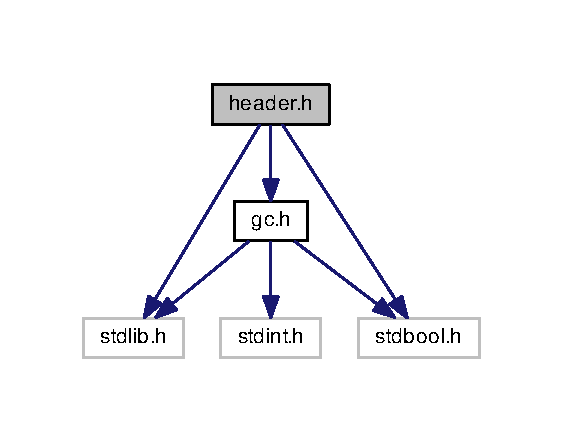
\includegraphics[width=270pt]{header_8h__incl}
\end{center}
\end{figure}
\subsection*{Typedefs}
\begin{DoxyCompactItemize}
\item 
\hypertarget{header_8h_ac6c34d4e6fbdfd05e85e560ba058f245}{typedef enum \hyperlink{header_8h_ad7f9678fbffaef587ba680031317a4f9}{header\-\_\-type} {\bfseries header\-\_\-type}}\label{header_8h_ac6c34d4e6fbdfd05e85e560ba058f245}

\end{DoxyCompactItemize}
\subsection*{Enumerations}
\begin{DoxyCompactItemize}
\item 
enum \hyperlink{header_8h_ad7f9678fbffaef587ba680031317a4f9}{header\-\_\-type} \{ \hyperlink{header_8h_ad7f9678fbffaef587ba680031317a4f9aa95b1e6d1fcdbcc145322e678f06f8dd}{R\-A\-W\-\_\-\-D\-A\-T\-A}, 
\hyperlink{header_8h_ad7f9678fbffaef587ba680031317a4f9a5f27f204111038192ec7c365d8a6a924}{S\-T\-R\-U\-C\-T\-\_\-\-R\-E\-P}, 
\hyperlink{header_8h_ad7f9678fbffaef587ba680031317a4f9aa0a820259add1d97da94e447ccc2d254}{F\-O\-R\-W\-A\-R\-D\-I\-N\-G\-\_\-\-A\-D\-D\-R}, 
\hyperlink{header_8h_ad7f9678fbffaef587ba680031317a4f9acfe24a7b308a82835c8a9a9a89bc4ca2}{N\-O\-T\-H\-I\-N\-G}
 \}
\begin{DoxyCompactList}\small\item\em The enumeration of different types a header can have. \end{DoxyCompactList}\end{DoxyCompactItemize}
\subsection*{Functions}
\begin{DoxyCompactItemize}
\item 
void $\ast$ \hyperlink{header_8h_a0b69fe045395358205ac6540a0c7b287}{create\-\_\-struct\-\_\-header} (\hyperlink{gc_8h_ad3bb09826584eab4757c6cd2f988e7d6}{heap\-\_\-t} $\ast$h, char $\ast$format\-\_\-string, void $\ast$heap\-\_\-ptr)
\begin{DoxyCompactList}\small\item\em Creates a header and saves it on the heap. \end{DoxyCompactList}\item 
void $\ast$ \hyperlink{header_8h_a2f4d174441c9fb8f2b62fb935256d912}{create\-\_\-data\-\_\-header} (size\-\_\-t bytes, void $\ast$heap\-\_\-ptr)
\begin{DoxyCompactList}\small\item\em Creates a header and saves it on the heap. \end{DoxyCompactList}\item 
\hyperlink{header_8h_ad7f9678fbffaef587ba680031317a4f9}{header\-\_\-type} \hyperlink{header_8h_a97a169b95fba1489a4810f5c9780dd56}{get\-\_\-header\-\_\-type} (void $\ast$)
\begin{DoxyCompactList}\small\item\em Gets the type of header belonging to the data. \end{DoxyCompactList}\item 
size\-\_\-t \hyperlink{header_8h_af484c9f937b9f91148b44e4801263ef0}{get\-\_\-number\-\_\-of\-\_\-pointers\-\_\-in\-\_\-struct} (void $\ast$structure)
\begin{DoxyCompactList}\small\item\em Get the number of pointers inside {\ttfamily structure}. \end{DoxyCompactList}\item 
bool \hyperlink{header_8h_a57105fa91cf9ef5bb4e88784675ccd96}{get\-\_\-pointers\-\_\-in\-\_\-struct} (void $\ast$structure, void $\ast$$\ast$array\mbox{[}$\,$\mbox{]})
\begin{DoxyCompactList}\small\item\em Finds all pointers inside {\ttfamily structure} and places pointers to them in {\ttfamily array}. \end{DoxyCompactList}\item 
size\-\_\-t \hyperlink{header_8h_ad1db70c039d8ccde85eb4c0ce43658b1}{get\-\_\-struct\-\_\-size} (char $\ast$format\-\_\-string)
\begin{DoxyCompactList}\small\item\em Calculates the size needed to store the structure represented by {\ttfamily format\-\_\-string}, including a header. \end{DoxyCompactList}\item 
size\-\_\-t \hyperlink{header_8h_a697872eb81c027c321904e10fabef050}{get\-\_\-data\-\_\-size} (size\-\_\-t bytes)
\begin{DoxyCompactList}\small\item\em Calculates the size needed to store data of size {\ttfamily bytes} with a header. \end{DoxyCompactList}\item 
size\-\_\-t \hyperlink{header_8h_a6951d82f26c04c88353d6368a14c20f8}{get\-\_\-existing\-\_\-size} (void $\ast$data)
\begin{DoxyCompactList}\small\item\em Get the size of data having a header. \end{DoxyCompactList}\item 
size\-\_\-t \hyperlink{header_8h_a27e0c278fd25a3520b2cc7755bdffaa4}{get\-\_\-existing\-\_\-data\-\_\-size} (void $\ast$data)
\begin{DoxyCompactList}\small\item\em Get the size of data having a header. \end{DoxyCompactList}\item 
void $\ast$ \hyperlink{header_8h_a9969f857712ff16735c160df84a711e0}{copy\-\_\-header} (void $\ast$data, void $\ast$heap\-\_\-ptr)
\begin{DoxyCompactList}\small\item\em Creates a copy of a header and saves the copy on the heap. \end{DoxyCompactList}\item 
bool \hyperlink{header_8h_af104ce328ab98be35be16611d39a0fe6}{forward\-\_\-header} (void $\ast$data, void $\ast$new\-\_\-data)
\begin{DoxyCompactList}\small\item\em forwards a header \end{DoxyCompactList}\item 
void $\ast$ \hyperlink{header_8h_a87def239dc6c8bda4dc44defc4d895de}{get\-\_\-forwarding\-\_\-address} (void $\ast$data)
\begin{DoxyCompactList}\small\item\em Gets the address that data has been forwarded to. \end{DoxyCompactList}\end{DoxyCompactItemize}


\subsection{Detailed Description}
A module for creating headers (meta data) for data and structures. \begin{DoxyAuthor}{Author}
Daniel Agstrand 

Henrik Bergendal 

Adam Inersjo 

Maria Lindqvist 

Simon Pellgard 

Robert Rosborg 
\end{DoxyAuthor}


\subsection{Enumeration Type Documentation}
\hypertarget{header_8h_ad7f9678fbffaef587ba680031317a4f9}{\index{header.\-h@{header.\-h}!header\-\_\-type@{header\-\_\-type}}
\index{header\-\_\-type@{header\-\_\-type}!header.h@{header.\-h}}
\subsubsection[{header\-\_\-type}]{\setlength{\rightskip}{0pt plus 5cm}enum {\bf header\-\_\-type}}}\label{header_8h_ad7f9678fbffaef587ba680031317a4f9}


The enumeration of different types a header can have. 

\begin{Desc}
\item[Enumerator]\par
\begin{description}
\index{R\-A\-W\-\_\-\-D\-A\-T\-A@{R\-A\-W\-\_\-\-D\-A\-T\-A}!header.\-h@{header.\-h}}\index{header.\-h@{header.\-h}!R\-A\-W\-\_\-\-D\-A\-T\-A@{R\-A\-W\-\_\-\-D\-A\-T\-A}}\item[{\em 
\hypertarget{header_8h_ad7f9678fbffaef587ba680031317a4f9aa95b1e6d1fcdbcc145322e678f06f8dd}{R\-A\-W\-\_\-\-D\-A\-T\-A}\label{header_8h_ad7f9678fbffaef587ba680031317a4f9aa95b1e6d1fcdbcc145322e678f06f8dd}
}]The header is followed by raw data \index{S\-T\-R\-U\-C\-T\-\_\-\-R\-E\-P@{S\-T\-R\-U\-C\-T\-\_\-\-R\-E\-P}!header.\-h@{header.\-h}}\index{header.\-h@{header.\-h}!S\-T\-R\-U\-C\-T\-\_\-\-R\-E\-P@{S\-T\-R\-U\-C\-T\-\_\-\-R\-E\-P}}\item[{\em 
\hypertarget{header_8h_ad7f9678fbffaef587ba680031317a4f9a5f27f204111038192ec7c365d8a6a924}{S\-T\-R\-U\-C\-T\-\_\-\-R\-E\-P}\label{header_8h_ad7f9678fbffaef587ba680031317a4f9a5f27f204111038192ec7c365d8a6a924}
}]The header is followed by data containing pointers \index{F\-O\-R\-W\-A\-R\-D\-I\-N\-G\-\_\-\-A\-D\-D\-R@{F\-O\-R\-W\-A\-R\-D\-I\-N\-G\-\_\-\-A\-D\-D\-R}!header.\-h@{header.\-h}}\index{header.\-h@{header.\-h}!F\-O\-R\-W\-A\-R\-D\-I\-N\-G\-\_\-\-A\-D\-D\-R@{F\-O\-R\-W\-A\-R\-D\-I\-N\-G\-\_\-\-A\-D\-D\-R}}\item[{\em 
\hypertarget{header_8h_ad7f9678fbffaef587ba680031317a4f9aa0a820259add1d97da94e447ccc2d254}{F\-O\-R\-W\-A\-R\-D\-I\-N\-G\-\_\-\-A\-D\-D\-R}\label{header_8h_ad7f9678fbffaef587ba680031317a4f9aa0a820259add1d97da94e447ccc2d254}
}]The header contains information about forwarded data \index{N\-O\-T\-H\-I\-N\-G@{N\-O\-T\-H\-I\-N\-G}!header.\-h@{header.\-h}}\index{header.\-h@{header.\-h}!N\-O\-T\-H\-I\-N\-G@{N\-O\-T\-H\-I\-N\-G}}\item[{\em 
\hypertarget{header_8h_ad7f9678fbffaef587ba680031317a4f9acfe24a7b308a82835c8a9a9a89bc4ca2}{N\-O\-T\-H\-I\-N\-G}\label{header_8h_ad7f9678fbffaef587ba680031317a4f9acfe24a7b308a82835c8a9a9a89bc4ca2}
}]There is no header \end{description}
\end{Desc}


\subsection{Function Documentation}
\hypertarget{header_8h_a9969f857712ff16735c160df84a711e0}{\index{header.\-h@{header.\-h}!copy\-\_\-header@{copy\-\_\-header}}
\index{copy\-\_\-header@{copy\-\_\-header}!header.h@{header.\-h}}
\subsubsection[{copy\-\_\-header}]{\setlength{\rightskip}{0pt plus 5cm}void$\ast$ copy\-\_\-header (
\begin{DoxyParamCaption}
\item[{void $\ast$}]{data, }
\item[{void $\ast$}]{heap\-\_\-ptr}
\end{DoxyParamCaption}
)}}\label{header_8h_a9969f857712ff16735c160df84a711e0}


Creates a copy of a header and saves the copy on the heap. 


\begin{DoxyParams}{Parameters}
{\em data} & the data containing the header to be copied \\
\hline
{\em heap\-\_\-ptr} & the place on the heap where the header will be saved \\
\hline
\end{DoxyParams}
\begin{DoxyReturn}{Returns}
pointer to where the data should be placed N\-U\-L\-L if {\ttfamily data} is N\-U\-L\-L or {\ttfamily heap\-\_\-ptr} is N\-U\-L\-L 
\end{DoxyReturn}
\hypertarget{header_8h_a2f4d174441c9fb8f2b62fb935256d912}{\index{header.\-h@{header.\-h}!create\-\_\-data\-\_\-header@{create\-\_\-data\-\_\-header}}
\index{create\-\_\-data\-\_\-header@{create\-\_\-data\-\_\-header}!header.h@{header.\-h}}
\subsubsection[{create\-\_\-data\-\_\-header}]{\setlength{\rightskip}{0pt plus 5cm}void$\ast$ create\-\_\-data\-\_\-header (
\begin{DoxyParamCaption}
\item[{size\-\_\-t}]{bytes, }
\item[{void $\ast$}]{heap\-\_\-ptr}
\end{DoxyParamCaption}
)}}\label{header_8h_a2f4d174441c9fb8f2b62fb935256d912}


Creates a header and saves it on the heap. 

This function is called when the header doesn't have to contain information about pointers existing inside data. The header created will be of the type R\-A\-W\-\_\-\-D\-A\-T\-A


\begin{DoxyParams}{Parameters}
{\em bytes} & the size in bytes \\
\hline
{\em heap\-\_\-ptr} & the place on the heap where the header will be saved \\
\hline
\end{DoxyParams}
\begin{DoxyReturn}{Returns}
pointer to where the data should be placed N\-U\-L\-L if {\ttfamily bytes} is zero or {\ttfamily heap\-\_\-ptr} is N\-U\-L\-L 
\end{DoxyReturn}
\hypertarget{header_8h_a0b69fe045395358205ac6540a0c7b287}{\index{header.\-h@{header.\-h}!create\-\_\-struct\-\_\-header@{create\-\_\-struct\-\_\-header}}
\index{create\-\_\-struct\-\_\-header@{create\-\_\-struct\-\_\-header}!header.h@{header.\-h}}
\subsubsection[{create\-\_\-struct\-\_\-header}]{\setlength{\rightskip}{0pt plus 5cm}void$\ast$ create\-\_\-struct\-\_\-header (
\begin{DoxyParamCaption}
\item[{{\bf heap\-\_\-t} $\ast$}]{h, }
\item[{char $\ast$}]{format\-\_\-string, }
\item[{void $\ast$}]{heap\-\_\-ptr}
\end{DoxyParamCaption}
)}}\label{header_8h_a0b69fe045395358205ac6540a0c7b287}


Creates a header and saves it on the heap. 

This function is called when the header is to be created for data represented by a format string. If there are pointers in the format string the header created will be of the type S\-T\-R\-U\-C\-T\-\_\-\-R\-E\-P, else it will be converted into R\-A\-W\-\_\-\-D\-A\-T\-A.

The {\ttfamily format\-\_\-string} will be copied and doesn't need to be placed on the heap before hand.


\begin{DoxyParams}{Parameters}
{\em h} & the heap to allocate {\ttfamily format\-\_\-string} in if it is too big \\
\hline
{\em format\-\_\-string} & the string representation of the structure to create a header for \\
\hline
{\em heap\-\_\-ptr} & the place on the heap where the header will be saved \\
\hline
\end{DoxyParams}
\begin{DoxyReturn}{Returns}
pointer to where the data should be placed 
\end{DoxyReturn}
\hypertarget{header_8h_af104ce328ab98be35be16611d39a0fe6}{\index{header.\-h@{header.\-h}!forward\-\_\-header@{forward\-\_\-header}}
\index{forward\-\_\-header@{forward\-\_\-header}!header.h@{header.\-h}}
\subsubsection[{forward\-\_\-header}]{\setlength{\rightskip}{0pt plus 5cm}bool forward\-\_\-header (
\begin{DoxyParamCaption}
\item[{void $\ast$}]{data, }
\item[{void $\ast$}]{new\-\_\-data}
\end{DoxyParamCaption}
)}}\label{header_8h_af104ce328ab98be35be16611d39a0fe6}


forwards a header 


\begin{DoxyParams}{Parameters}
{\em data} & the data containing the header to be forwarded \\
\hline
{\em new\-\_\-data} & the data the header will be forwarded to \\
\hline
\end{DoxyParams}
\begin{DoxyReturn}{Returns}
true if the forwarding was successfull, false otherwise 
\end{DoxyReturn}
\hypertarget{header_8h_a697872eb81c027c321904e10fabef050}{\index{header.\-h@{header.\-h}!get\-\_\-data\-\_\-size@{get\-\_\-data\-\_\-size}}
\index{get\-\_\-data\-\_\-size@{get\-\_\-data\-\_\-size}!header.h@{header.\-h}}
\subsubsection[{get\-\_\-data\-\_\-size}]{\setlength{\rightskip}{0pt plus 5cm}size\-\_\-t get\-\_\-data\-\_\-size (
\begin{DoxyParamCaption}
\item[{size\-\_\-t}]{bytes}
\end{DoxyParamCaption}
)}}\label{header_8h_a697872eb81c027c321904e10fabef050}


Calculates the size needed to store data of size {\ttfamily bytes} with a header. 


\begin{DoxyParams}{Parameters}
{\em bytes} & the size of the data \\
\hline
\end{DoxyParams}
\begin{DoxyReturn}{Returns}
the size needed for storing the data with a header. If {\ttfamily bytes} combined with the size of the header extends maximum size for size\-\_\-t the function will return 0. Zero is also returned when {\ttfamily bytes} is 0. 
\end{DoxyReturn}
\hypertarget{header_8h_a27e0c278fd25a3520b2cc7755bdffaa4}{\index{header.\-h@{header.\-h}!get\-\_\-existing\-\_\-data\-\_\-size@{get\-\_\-existing\-\_\-data\-\_\-size}}
\index{get\-\_\-existing\-\_\-data\-\_\-size@{get\-\_\-existing\-\_\-data\-\_\-size}!header.h@{header.\-h}}
\subsubsection[{get\-\_\-existing\-\_\-data\-\_\-size}]{\setlength{\rightskip}{0pt plus 5cm}size\-\_\-t get\-\_\-existing\-\_\-data\-\_\-size (
\begin{DoxyParamCaption}
\item[{void $\ast$}]{data}
\end{DoxyParamCaption}
)}}\label{header_8h_a27e0c278fd25a3520b2cc7755bdffaa4}


Get the size of data having a header. 

The size of the header itself is N\-O\-T included in the result


\begin{DoxyParams}{Parameters}
{\em data} & pointer to the data to get size of \\
\hline
\end{DoxyParams}
\begin{DoxyReturn}{Returns}
size of data 
\end{DoxyReturn}
\hypertarget{header_8h_a6951d82f26c04c88353d6368a14c20f8}{\index{header.\-h@{header.\-h}!get\-\_\-existing\-\_\-size@{get\-\_\-existing\-\_\-size}}
\index{get\-\_\-existing\-\_\-size@{get\-\_\-existing\-\_\-size}!header.h@{header.\-h}}
\subsubsection[{get\-\_\-existing\-\_\-size}]{\setlength{\rightskip}{0pt plus 5cm}size\-\_\-t get\-\_\-existing\-\_\-size (
\begin{DoxyParamCaption}
\item[{void $\ast$}]{data}
\end{DoxyParamCaption}
)}}\label{header_8h_a6951d82f26c04c88353d6368a14c20f8}


Get the size of data having a header. 

The size of the header itself is included in the result


\begin{DoxyParams}{Parameters}
{\em data} & pointer to the data to get size of \\
\hline
\end{DoxyParams}
\begin{DoxyReturn}{Returns}
size of data combined with header 
\end{DoxyReturn}
\hypertarget{header_8h_a87def239dc6c8bda4dc44defc4d895de}{\index{header.\-h@{header.\-h}!get\-\_\-forwarding\-\_\-address@{get\-\_\-forwarding\-\_\-address}}
\index{get\-\_\-forwarding\-\_\-address@{get\-\_\-forwarding\-\_\-address}!header.h@{header.\-h}}
\subsubsection[{get\-\_\-forwarding\-\_\-address}]{\setlength{\rightskip}{0pt plus 5cm}void$\ast$ get\-\_\-forwarding\-\_\-address (
\begin{DoxyParamCaption}
\item[{void $\ast$}]{data}
\end{DoxyParamCaption}
)}}\label{header_8h_a87def239dc6c8bda4dc44defc4d895de}


Gets the address that data has been forwarded to. 


\begin{DoxyParams}{Parameters}
{\em data} & the data containing the header to get forwarding address from \\
\hline
\end{DoxyParams}
\begin{DoxyReturn}{Returns}
the address where {\ttfamily data} has been forwarded to N\-U\-L\-L if {\ttfamily data} isn't of type F\-O\-R\-W\-A\-R\-D\-I\-N\-G\-\_\-\-A\-D\-D\-R 
\end{DoxyReturn}
\hypertarget{header_8h_a97a169b95fba1489a4810f5c9780dd56}{\index{header.\-h@{header.\-h}!get\-\_\-header\-\_\-type@{get\-\_\-header\-\_\-type}}
\index{get\-\_\-header\-\_\-type@{get\-\_\-header\-\_\-type}!header.h@{header.\-h}}
\subsubsection[{get\-\_\-header\-\_\-type}]{\setlength{\rightskip}{0pt plus 5cm}{\bf header\-\_\-type} get\-\_\-header\-\_\-type (
\begin{DoxyParamCaption}
\item[{void $\ast$}]{}
\end{DoxyParamCaption}
)}}\label{header_8h_a97a169b95fba1489a4810f5c9780dd56}


Gets the type of header belonging to the data. 

The available types are F\-O\-R\-W\-A\-R\-D\-I\-N\-G\-\_\-\-A\-D\-D\-R, S\-T\-R\-U\-C\-T\-\_\-\-R\-E\-P and R\-A\-W\-\_\-\-D\-A\-T\-A.


\begin{DoxyParams}{Parameters}
{\em data} & the data to analyze \\
\hline
\end{DoxyParams}
\begin{DoxyReturn}{Returns}
the type of header beloning to {\ttfamily data}, N\-O\-T\-H\-I\-N\-G if {\ttfamily data} is N\-U\-L\-L 
\end{DoxyReturn}
\hypertarget{header_8h_af484c9f937b9f91148b44e4801263ef0}{\index{header.\-h@{header.\-h}!get\-\_\-number\-\_\-of\-\_\-pointers\-\_\-in\-\_\-struct@{get\-\_\-number\-\_\-of\-\_\-pointers\-\_\-in\-\_\-struct}}
\index{get\-\_\-number\-\_\-of\-\_\-pointers\-\_\-in\-\_\-struct@{get\-\_\-number\-\_\-of\-\_\-pointers\-\_\-in\-\_\-struct}!header.h@{header.\-h}}
\subsubsection[{get\-\_\-number\-\_\-of\-\_\-pointers\-\_\-in\-\_\-struct}]{\setlength{\rightskip}{0pt plus 5cm}size\-\_\-t get\-\_\-number\-\_\-of\-\_\-pointers\-\_\-in\-\_\-struct (
\begin{DoxyParamCaption}
\item[{void $\ast$}]{structure}
\end{DoxyParamCaption}
)}}\label{header_8h_af484c9f937b9f91148b44e4801263ef0}


Get the number of pointers inside {\ttfamily structure}. 

The function will only return valid information if a struct\-\_\-header has been created and placed just before the struct in the heap.


\begin{DoxyParams}{Parameters}
{\em structure} & the structure to look for pointers in \\
\hline
\end{DoxyParams}
\begin{DoxyReturn}{Returns}
number of pointers found in {\ttfamily structure} if its header has the type S\-T\-R\-U\-C\-T\-\_\-\-R\-E\-P. Otherwise it will return 0 
\end{DoxyReturn}
\hypertarget{header_8h_a57105fa91cf9ef5bb4e88784675ccd96}{\index{header.\-h@{header.\-h}!get\-\_\-pointers\-\_\-in\-\_\-struct@{get\-\_\-pointers\-\_\-in\-\_\-struct}}
\index{get\-\_\-pointers\-\_\-in\-\_\-struct@{get\-\_\-pointers\-\_\-in\-\_\-struct}!header.h@{header.\-h}}
\subsubsection[{get\-\_\-pointers\-\_\-in\-\_\-struct}]{\setlength{\rightskip}{0pt plus 5cm}bool get\-\_\-pointers\-\_\-in\-\_\-struct (
\begin{DoxyParamCaption}
\item[{void $\ast$}]{structure, }
\item[{void $\ast$$\ast$}]{array\mbox{[}$\,$\mbox{]}}
\end{DoxyParamCaption}
)}}\label{header_8h_a57105fa91cf9ef5bb4e88784675ccd96}


Finds all pointers inside {\ttfamily structure} and places pointers to them in {\ttfamily array}. 

The function will only return valid information if a struct\-\_\-header has been created and placed just before the struct in the heap.

{\ttfamily structure} has to have the header type Structure\-\_\-rep. {\ttfamily array} must be of size get\-\_\-numer\-\_\-of\-\_\-pointers\-\_\-in\-\_\-structure({\ttfamily structure}).


\begin{DoxyParams}{Parameters}
{\em structure} & the structure to look for pointers is \\
\hline
{\em array} & the array to place pointers to the pointers found in header of {\ttfamily structure} \\
\hline
\end{DoxyParams}
\begin{DoxyReturn}{Returns}
true if pointers were found and placed in {\ttfamily array}, false otherwise 
\end{DoxyReturn}
\hypertarget{header_8h_ad1db70c039d8ccde85eb4c0ce43658b1}{\index{header.\-h@{header.\-h}!get\-\_\-struct\-\_\-size@{get\-\_\-struct\-\_\-size}}
\index{get\-\_\-struct\-\_\-size@{get\-\_\-struct\-\_\-size}!header.h@{header.\-h}}
\subsubsection[{get\-\_\-struct\-\_\-size}]{\setlength{\rightskip}{0pt plus 5cm}size\-\_\-t get\-\_\-struct\-\_\-size (
\begin{DoxyParamCaption}
\item[{char $\ast$}]{format\-\_\-string}
\end{DoxyParamCaption}
)}}\label{header_8h_ad1db70c039d8ccde85eb4c0ce43658b1}


Calculates the size needed to store the structure represented by {\ttfamily format\-\_\-string}, including a header. 


\begin{DoxyParams}{Parameters}
{\em format\-\_\-string} & the string representation of a structure \\
\hline
\end{DoxyParams}
\begin{DoxyReturn}{Returns}
the size needed for the structure 
\end{DoxyReturn}

\hypertarget{stack__search_8h}{\section{stack\-\_\-search.\-h File Reference}
\label{stack__search_8h}\index{stack\-\_\-search.\-h@{stack\-\_\-search.\-h}}
}


A module for searching through the stack.  


\subsection*{Functions}
\begin{DoxyCompactItemize}
\item 
void $\ast$$\ast$ \hyperlink{stack__search_8h_a602e1757a197da5dbd6402a7ce335fad}{stack\-\_\-find\-\_\-next\-\_\-ptr} (void $\ast$$\ast$stack\-\_\-bottom, void $\ast$stack\-\_\-top, void $\ast$heap\-\_\-start, void $\ast$heap\-\_\-end)
\begin{DoxyCompactList}\small\item\em Finds a possible pointer on the stack. \end{DoxyCompactList}\end{DoxyCompactItemize}


\subsection{Detailed Description}
A module for searching through the stack. \begin{DoxyAuthor}{Author}
Daniel Agstrand 

Henrik Bergendal 

Adam Inersjo 

Maria Lindqvist 

Simon Pellgard 

Robert Rosborg 
\end{DoxyAuthor}


\subsection{Function Documentation}
\hypertarget{stack__search_8h_a602e1757a197da5dbd6402a7ce335fad}{\index{stack\-\_\-search.\-h@{stack\-\_\-search.\-h}!stack\-\_\-find\-\_\-next\-\_\-ptr@{stack\-\_\-find\-\_\-next\-\_\-ptr}}
\index{stack\-\_\-find\-\_\-next\-\_\-ptr@{stack\-\_\-find\-\_\-next\-\_\-ptr}!stack_search.h@{stack\-\_\-search.\-h}}
\subsubsection[{stack\-\_\-find\-\_\-next\-\_\-ptr}]{\setlength{\rightskip}{0pt plus 5cm}void$\ast$$\ast$ stack\-\_\-find\-\_\-next\-\_\-ptr (
\begin{DoxyParamCaption}
\item[{void $\ast$$\ast$}]{stack\-\_\-bottom, }
\item[{void $\ast$}]{stack\-\_\-top, }
\item[{void $\ast$}]{heap\-\_\-start, }
\item[{void $\ast$}]{heap\-\_\-end}
\end{DoxyParamCaption}
)}}\label{stack__search_8h_a602e1757a197da5dbd6402a7ce335fad}


Finds a possible pointer on the stack. 


\begin{DoxyParams}{Parameters}
{\em stack\-\_\-bottom} & the bottom of the stack to seach \\
\hline
{\em stack\-\_\-top} & the top of the stack to seach \\
\hline
{\em heap\-\_\-start} & the start of the heap \\
\hline
{\em heap\-\_\-end} & the last position in the heap to which a pointer is allowed to refer \\
\hline
\end{DoxyParams}
\begin{DoxyReturn}{Returns}
a pointer to a location in the stack between {\ttfamily stack\-\_\-bottom} and {\ttfamily stack\-\_\-top} that contains a possible address into the heap between {\ttfamily heap\-\_\-start} and {\ttfamily heap\-\_\-end}, or N\-U\-L\-L if search is finished
\end{DoxyReturn}
Before calling stack search registers need to be dumped to the stack. This can be achieved by\-: \#include $<$setjmp.\-h$>$ \#define Dump\-\_\-registers() \textbackslash{} jmp\-\_\-buf env; \textbackslash{} if (setjmp(env)) abort(); \textbackslash{}

When calling the function use; \-\_\-\-\_\-builtin\-\_\-frame\-\_\-address(n); To get a pointer to the start of a scopes memory on stack. $<$n$>$ specifies what scope. 0 is the current, 1 the one above. On S\-P\-A\-R\-C with Sun C Compiler this doesn't work so another method is needed.

extern char $\ast$$\ast$environ; To get the bottom of the programs' stack. When refering to it use something similar to\-: void $\ast$stack\-\_\-bottom = (void $\ast$)$\ast$environ; void $\ast$pointer = stack\-\_\-find\-\_\-next\-\_\-ptr(\&stack\-\_\-bottom, stack\-\_\-top, heap\-\_\-start, heap\-\_\-end); 
%--- End generated contents ---

% Index
\backmatter
\newpage
\phantomsection
\clearemptydoublepage
\addcontentsline{toc}{chapter}{Index}
\printindex

\end{document}
